\documentclass[a4paper,12pt]{article}
\usepackage[utf8]{inputenc}
\usepackage[margin=2cm]{geometry}
\usepackage{enumitem}
\usepackage{amsmath}
\usepackage{amsthm}
\usepackage{mathtools}
\newtheorem{lemma}{Lemma}
\newtheorem{theorem}{Theorem}
\usepackage{amssymb}
\usepackage[english]{babel}
\usepackage{filecontents}
\usepackage{csquotes}
\usepackage{graphicx}
\usepackage{tikz}
\usetikzlibrary{bending}

\usepackage[colorlinks=false]{hyperref}
\usepackage[backend=bibtex,style=chem-angew,citestyle=numeric-comp,articletitle=true,hyperref=true,url=true]{biblatex}
\addbibresource{biblio.bib}
\usepackage{titlesec}
\usepackage{tocloft}

\begin{filecontents}{biblio.bib}
@article{Itai1990,
  doi = {10.1016/0890-5401(90)90004-2},
  url = {https://doi.org/10.1016/0890-5401(90)90004-2},
  year = {1990},
  month = sep,
  publisher = {Elsevier {BV}},
  volume = {88},
  number = {1},
  pages = {60--87},
  author = {Alon Itai and Michael Rodeh},
  title = {Symmetry breaking in distributed networks},
  journal = {Information and Computation}
}
\end{filecontents}


\begin{document}
\section{Size estimation in anonymous directed rings}
Itai and Rodeh \cite{Itai1990} proposed a probabilistic distributed algorithm for estimating the size of an anonymous directed ring with asynchronous message-passing communication. The algorithm is based on performing tests on successive ring size estimates, using random identifiers for symmetry breaking. The ring size algorithm is necessarily Monte Carlo, i.e. it contains finite executions in which an incorrect ring size is computed.

\section{The algorithm}
Each node $v$ maintains an estimate $est_{v}$ of the ring size; initially $est_{v} = 1$. Throughout the execution of the algorithm, $est_{v}$ will never exceed the ring size $n$. Each node proceeds in rounds. Each time a node finds that its estimate is too conservative, it moves to another round and increases its estimate accordingly.

Each round, $v$ randomly chooses an ID $id_{v}$ and sends the message $(est_{v},id_{v},1)$ to its neighbor. The third value is a hop count that increases by one each time the message is forwarded. The node hopes that the message will be forwarded to distance $est_{v}$, and in a case where $est_{v} = n$, the message will complete a round trip and return. However, during the forwarding process, intermediate nodes may decide to purge messages, update their own estimates and/or send new messages based on the message contents.

Now $v$ waits for a message $(est,id,h)$ to arrive. An invariant of such messages is that $h\leq est$ always holds. When a message arrives, $v$ acts as follows, depending on the message contents.

\begin{enumerate}
\item $est < est_{v}$: The estimate of the message is more conservative than the estimate of $v$, so $v$ purges the message.
\item $est \geq est_{v} \land h < est$: The estimate $est$ may be correct. So $v$ sends $(est,id,h+1)$ to give the message a chance to complete its round-trip. If $est_{v} < est$, $v$ performs $est_{v}\leftarrow est$ to make sure not to accept smaller estimates in the future.\label{itm:case-forwarding}
\item $est \geq est_{v} \land h=est$:
\begin{enumerate}
\item $est > est_{v} \lor id \neq id_{v}$: The estimate $est$ is too conservative because the message travelled $est$ hops but did not complete its round trip. So $v$ performs $est_{v}\leftarrow est+1$.
\item $est = est_{v} \land id = id_{v}$: This message is indistinguishable from $v$'s own message. It is either $v$'s own message, or a message from a node $est$ hops before $v$ that happened to select the same ID as $v$. In this case $v$'s confidence in the estimate $est_{v}$ increases.\label{itm:case-all-checks-passed}
\end{enumerate}
\end{enumerate}

A node achieves full confidence in a given estimate once it has recorded a total of r messages satisfying the case \ref{itm:case-all-checks-passed}, where $r$ is an algorithm parameter. It will then send a termination message around the ring. The algorithm may terminate with an estimate less than $n$ if too many false positives are recorded.

\section{Correctness and complexity}

\begin{theorem}
Throughout the execution of the algorithm $h \leq est \leq n$ Also, $est_v\leq n$.
\end{theorem}
\begin{proof}
Initially $est_v = 1 \leq n$.
Each new message is initiated with $h = 1 \leq est$.
Messages with $h=est$ are never forwarded.
Estimates are only increased if they are certain to be too conservative.
\end{proof}

\begin{theorem}
At most $O(rn^3)$ messages will be sent during the execution of the algorithm.
\end{theorem}
\begin{proof}
Each of the $n$ nodes will consider at most $n$ different estimates. When verifying an estimate, a node will produce at most $r$ new messages (those with hop count 1). Each of these messages will travel at most $n$ steps.
\end{proof}
Note that this is a very rough estimate, and in practice the number of messages is much lower.

\section{Context}

\begin{theorem}
\label{thm:no-las-vegas-ring-size-algorithm}
There is no Las Vegas algorithm for computing the size of an anonymous ring.
\end{theorem}
\begin{proof}
Suppose we have an algorithm for computing the size of an anonymous ring of size $n$, with nodes $v_0,\dots,v_{n-1}$.
Let $E$ be a finite execution of this algorithm that gives the correct answer $n$.
Cut the ring in half, make a copy of it, and then glue two copies together so that the node $v_0$ is connected to the node $v_{n-1}'$ and $v_0'$ is connected to $v_{n-1}$.
That is, we consider the anonymous ring of size $2n$ shown in \ref{fig:ring}.
Now define $E'$ as replaying $E$ twice, simultaneously, on the resulting ring. Once on the half $v_0,\dots,v_{n-1}$, where $v_0$ communicates with $v_{n-1}'$ instead of $v_{n-1}$, and once on the half $v_0',\dots,v_{n-1}'$, where $v_{n-1}'$ communicates with $v_0$.
Since the ring is anonymous, nodes cannot tell the difference between participating in $E$ on a ring of size $n$ and participating in $E'$ on a ring of size $2n$. In $E'$ all nodes terminate with the wrong result $n$.
This reasoning can be adapted to undirected rings as well.

\begin{figure}
\centering
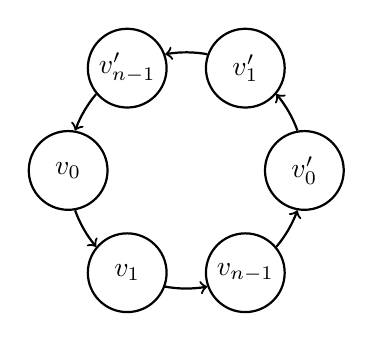
\begin{tikzpicture}[
  ->,   
  thick,
  main node/.style={circle, draw, minimum size=1cm},
]
  \newcommand*{\MainNum}{6}
  \newcommand*{\MainRadius}{1.5cm} 
  \newcommand*{\MainStartAngle}{180}

  % Print main nodes, node names: p1, p2, ...
  \path
    (0, 0) coordinate (M)
    \foreach \t [count=\i] in {$v_0$, $v_1$, $v_{n-1}$, $v_0'$, $v_1'$, $v_{n-1}'$} {
      +({\i-1)*360/\MainNum + \MainStartAngle}:\MainRadius)
      node[main node, label=center:\t] (p\i) {}
    }
  ;  

  % Calculate the angle between the equal sides of the triangle
  % with side length \MainRadius, \MainRadius and radius of circle node
  % Result is stored in \p1-angle, \p2-angle, ...
  \foreach \i in {1, ..., \MainNum} {
    \pgfextracty{\dimen0 }{\pgfpointanchor{p\i}{north}} 
    \pgfextracty{\dimen2 }{\pgfpointanchor{p\i}{center}}
    \dimen0=\dimexpr\dimen2 - \dimen0\relax 
    \ifdim\dimen0<0pt \dimen0 = -\dimen0 \fi
    \pgfmathparse{2*asin(\the\dimen0/\MainRadius/2)}
    \global\expandafter\let\csname p\i-angle\endcsname\pgfmathresult
  }

  % Draw the arrow arcs
  \foreach \i [evaluate=\i as \nexti using {int(mod(\i, \MainNum)+1}]
  in {1, ..., \MainNum} {  
    \pgfmathsetmacro\StartAngle{   
      (\i-1)*360/\MainNum + \MainStartAngle
      + \csname p\i-angle\endcsname
    }
    \pgfmathsetmacro\EndAngle{
      (\nexti-1)*360/\MainNum + \MainStartAngle
      - \csname p\nexti-angle\endcsname
    }
    \ifdim\EndAngle pt < \StartAngle pt
      \pgfmathsetmacro\EndAngle{\EndAngle + 360}
    \fi
    \draw
      (M) ++(\StartAngle:\MainRadius)
      arc[start angle=\StartAngle, end angle=\EndAngle, radius=\MainRadius]
    ;
  }
\end{tikzpicture}
\caption{Two ring copies glued together}\label{fig:ring}
\end{figure}
\end{proof}

\begin{theorem}
There is no Las Vegas algorithm for leader election in anonymous rings when nodes do not know the ring size.
\end{theorem}
\begin{proof}
If such an algorithm existed, the leader, once elected, could determine the ring size by initiating a traversal algorithm. This would be a contradiction with \ref{thm:no-las-vegas-ring-size-algorithm}.
\end{proof}

\section{Notes}
My description of the algorithm differs slightly from the original.

\begin{itemize}
    \item In the original implementation, in the case \ref{itm:case-forwarding}, when setting $est_v \leftarrow est$, $v$ would send a message initialising a new round. This can be omitted, as $v$ is sure that messages with estimates not less than $est_v$ are travelling around the ring (such message was just forwarded, after all). Therefore $v$ can wait for further messages. This change reduces the execution time considerably.
    \item In the original implementation, the initial estimate is set to $2$, but dropping it to $1$ has no effect on the algorithm.
    \item In the original implementation, there is no explicit mention of the termination messages. It is only mentioned that the messages will stop being generated at some point.
\end{itemize}

\printbibliography
\end{document}
